
%----------------------------------------------------------------------------------------
%	PACKAGES AND THEMES
%----------------------------------------------------------------------------------------
\documentclass[aspectratio=169,xcolor=dvipsnames,handout]{beamer}
\usetheme{Darmstadt}
\usecolortheme{seahorse}

\usepackage[hangul]{kotex}

\usepackage{hyperref}
\usepackage{amsfonts, amssymb}
\usepackage{graphicx} % Allows including images
\usepackage{array, booktabs, multicol, multirow, tabularx} % Allows the use of \toprule, \midrule and \bottomrule in tables
\setbeamercovered{transparent}

\newcommand{\R}{\mathbb{R}}
\newcommand{\y}{\mathbf{y}}

%----------------------------------------------------------------------------------------
%	TITLE PAGE
%----------------------------------------------------------------------------------------

\title[좌파적 자유주의]{좌파적 자유주의} % The short title appears at the bottom of every slide, the full title is only on the title page
\subtitle{경제정의와 불평등}

\author[오성재]{오성재}

\institute[HNU] % Your institution as it will appear on the bottom of every slide, may be shorthand to save space
{
    한남대학교 \\
    탈메이지 교양학부 \\
}
\date{\today} % Date, can be changed to a custom date


%----------------------------------------------------------------------------------------
%	PRESENTATION SLIDES
%----------------------------------------------------------------------------------------

\begin{document}

\begin{frame}
    \titlepage
\end{frame}

\begin{frame}{목차}
    \tableofcontents
\end{frame}

\section{들어가늘 말}

\begin{frame}[<+->]
\frametitle{좌파적 자유주의}
    \begin{itemize}
        \item 로크, 루소, 칸트로 이어지는 고전 사회계약 이론을 일반화하면서 더 높은 수준의 추상화를 접목.
        \item 공리주의에 대한 합리적이고 체계적인 대안을 제공하는 정의의 개념 제시.
    \end{itemize}
\end{frame}

\begin{frame}[<+->]
\frametitle{존 롤즈}
    \begin{columns}
        \begin{column}{.5\textwidth}
            \begin{figure}
                \centering
                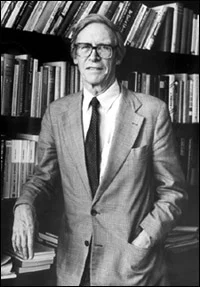
\includegraphics[width=.5\textwidth]{pic/Rawls_portrait.png}
            \end{figure}
        \end{column}    
        \begin{column}{.5\textwidth}
            \begin{itemize}
            \item John Rawls 
            \item 1921. 2. 21 - 2002. 11. 24
            \item 미국인 철학자
            \item 대표저서 : 정의론(A theory of justice)
            \end{itemize}
        \end{column}    
    \end{columns}
\end{frame}

\begin{frame}[<+->]
\frametitle{공리주의(utilitarianism)에 대한 롤즈의 비판}
    \begin{itemize}
        \item \textbf{사회}를 단순히 효용(의 구성 요소)의 생산활동을 위한 공동체로 간주.
        \item 사회 구성원인 \textbf{개인}을 일차적으로 효용의 수단으로 간주.
        \item 효용의 총합에만 초점을 맞추므로 자원, 기회, 부담 및 권리가 \textbf{어떻게} 분배되어야 하는지에 대한 설명 부족.
        \item 개인의 효용 추구에서 어떤 \textbf{기본권}이 중요한 데 공리주의는 이를 파악하지 못하고, 따라서 그 기본권을 모두에게 동등하게 보호하지 못함.
    \end{itemize}
\end{frame}
 
\begin{frame}[<+->]
\frametitle{롤즈 vs. 하이에크}
    \begin{itemize}
        \item 롤즈와 하이에크는 분배적 정의의 원칙과 이를 실현할 사회체제의 관계가 서로 상반됨.
        \begin{itemize}
            \item  롤즈는 민주사회가 정의로운 사회이고 이를 이루기 위해 분배적 정의의 원칙을 제시. 
            \item  하이에크는 정의로운 분배를 달성하기 위한 수단으로 자유시장주의와 법치주의가 필요하다는 입장. 
        \end{itemize}
    \end{itemize}
\end{frame}

\begin{frame}[<+->]
\frametitle{사회계약론}
    \begin{itemize}
        \item 공리주의에 대한 사회계약론적 대안 탐색
        \item 사회계약론에서 정치적 권위는 권위에 구속되는 구성원들의 동의에 기반. 
        \item 동의에 대한 두 가지 입장이 존재 :
        \begin{itemize}
            \item 동의는 실질적이므로 정치적 권위는 헌법과 같은 실제 사회적 계약에 의해 생성된 경우에만 합법적.
            \item 동의는 가상적이어서 모든 시민이 사회 계약에서 동의할 수 있는 원칙에 따라 정치적 권위가 행사되는 경우 합법적.
        \end{itemize}
    \end{itemize}
\end{frame}

\begin{frame}[<+->]
\frametitle{롤즈의 사회계약론}
    \begin{itemize}
        \item 롤즈는 가상적 동의의 개념하에, 모든 시민이 정치제도 및 법률 시스템의 설계 및 실행에 대한 권위 있고 동의할 수 있는 원칙을 찾으려고 함.
        \item 롤즈의 정의론은 민주사회와 민주시민의식에 대한 사상.
        \item 민주주의 사회에서 가장 좋은 정의의 개념에 대한 탐구.
    \end{itemize}
\end{frame}

\section{민주사회(democratic society)를 위한 정의}
\begin{frame}[<+->]
\frametitle{정의의 개념}
    \begin{itemize}
        \item 정의의 개념은 옳고 그름과 관련된 사고 영역(옮음, 가치 , 도덕 등)의 일부.
        \begin{itemize}
            \item 옮음 : 적절하고 동기가 부여된 당사자들이 동의하는 것으로 이해되어야.
        \end{itemize}
        \begin{itemize}
            \item  정의의 역할은 사회적 협력의 공정한 조건을 명시함으로써 구성원이 사회의 법과 제도 선택하도록 돕는 것.
            \item  정의의 주제(subject)는 기본적인 권리와 의무를 정의하는 제도와 법 체계. 
            \begin{itemize}
                \item 직위와 권력에 대한 접근. 
                \item 재산, 계약 및 기타 경제적 권리의 제정.
                \item 과세, 상속 및 유산에 관한 법률.
                \item 의료, 교육 및 사회의 다른 많은 재화에 대한 접근을 정의하는 규칙.
            \end{itemize}
        \end{itemize}
        \item  정의의 기본 형태는 (간단히 말해) 공정성.
    \end{itemize}
\end{frame}

\begin{frame}[<+->]
\frametitle{정의의 상황(circumstance)}
    \begin{itemize}
        \item 정의는 특정 상황에서만 유효. 
        \item 흄(Hume, D.)은 정의의 출현을 필요로 하는 상황은 크게 객관적인 상황과 주관적인 상황으로 구분.
        \begin{itemize}
            \item 객관적인 상황 : 적당한 희소성과 사람들 사이의 상호 작용. 
            \item 주관적인 상황 : 인간 본성에 있는 이기심과 제한적인 관대함.
        \end{itemize}
        \item 인간의 본성에서 관대함이나 동정심이 부족 or 분배대상인 자원이 부족하거나 협력이 불가능 $\rightarrow$ 정의의 실현 불가능.
        \item 인간의 본성이 지나치게 동정적이거나 자비로움 or 자원이 지나치게 풍부한 경우 $\rightarrow$ 정의는 아무 소용이 없음.
    \end{itemize}
\end{frame}



\begin{frame}[<+->]
\frametitle{정의의 상황(circumstance)}
    \begin{itemize}
        \item  롤스는 다양한 원칙들이 공존하는 다원주의가 민주주의 사회의 영구적인 특징이라는 "다원주의의 사실"을 추가.
        \begin{itemize}
            \item 종교, 철학, 삶의 의미, 그리고 그 자체로 추구할 가치가 있는 목적에 대한 불일치는 민주주의 사회의 영구적인 특징.
            \item 포괄적인 원칙에 대한 사회적 합의는 강압적인 국가 권력을 통해서만 확립.
        \end{itemize}
    \end{itemize}
\end{frame}

\begin{frame}[<+->]
\frametitle{정의의 상황(circumstance)}
    \begin{itemize}
        \item 다원주의 사실하에 정의의 개념은 강압적인 국가 권력의 사용이 필요함.
        \begin{itemize}
            \item  그러나 강압적인 국가권력의 남용은 자유주의 원칙에 위배.
            \item  "정치적 권력행사는 정치적 행동의 근거가 다른 시민들에게 (그러한 행동에 대한) 정당화로 합리적으로 받아들여질 수 있다고 진심으로 믿을 때에만 비로소 적절하다."
        \end{itemize}
    \item 강압적인 국가 권력의 필요성에 또다른 근거는 민주주의 사회와 공동체 간의 차이에서 찾을 수 있음.
    \begin{itemize}
        \item 공동체는 공유된 신념(예: 교회)하에 공동의 목적을 위해 연합하고 함께 일하는 사람들의 모임.
        \item 민주주의 사회는 특정한 목적에 대한 이러한 종류의 공유를 할 수 없고 해서도 안됨.
        \item 왜냐하면 올바른 목적이 무엇인지에 대해 시민들 사이에 합리적인 불일치가 있을 것이고, 이때의 합의는 정치적 강제의 불법적 사용을 통해서만 가능하기 때문.
    \end{itemize}
    \end{itemize}
\end{frame}

\begin{frame}[<+->]
\frametitle{정의의 형식적 제약}
    \begin{itemize}
        \item  롤즈는 정의의 개념이 충족해야 하는 다섯 가지 제약을 제시.
        \begin{itemize}
            \item  일반성 : 원칙은 일반적이어야. 
            \item  보편성 : 원칙은 보편적으로 적용되어야.
            \item  질서 : 원칙은 상충되는 주장을 정렬해야 하며, 시민이 제기할 수 있는 다양한 주장을 판결하기 위한 원칙적인 근거를 제공. 
            \item  최종성 : 원칙은 상충되는 주장에 대한 협상에서 최종 법원의 역할을 해야.
            \item  대중성 : 모든 구성원이 그들 사이의 공개 합의의 결과인 것처럼 기꺼이 수락하고 행동할 수 있어야.
        \end{itemize}
        \item  정의의 개념은 형식이 일반적이고 적용이 보편적인 일련의 원칙으로, 도덕적인 사람들의 상충되는 주장을 명령하기 위한 최종 법원으로 공개적으로 인정되어야 한다.
    \end{itemize}
\end{frame}


\begin{frame}[<+->]
\frametitle{정의의 후보 개념}
    \begin{itemize}
        \item  정의의 후보 개념은 정의의 개념을 잘 담고 있는 정의에 대한 원칙들.
        \begin{itemize}
            \item 공리주의, 완벽주의, 공산주의, 자유지상주의 등 널리 알려진 정의에 대한 모든 원칙들이 포함.
            \item 후보 개념에 대한 유일한 제약은 옳음의 개념의 형식적 제약을 충족할 수 있어야 한다는 점.
        \end{itemize}
        \item  다음의 세 종류의 이기주의는 정의의 후보개념에 포함되지 않음.
        \begin{itemize}
            \item 일인 독재 : 모두가 나의 이익에 부합해야 함.
            \item 무임승차 이기주의 : 내가 아닌 모든 사람은 정당하게 행동해야 함.
            \item 일반적 이기주의 : 모두가 원하는 대로 각자 이익을 추구해야 함.
        \end{itemize}
    \end{itemize}
\end{frame}

\begin{frame}[<+->]
\frametitle{질서있는 사회(Well-Ordered Societies)}
    \begin{itemize}
        \item  정의의 후보 개념이 형식적 제약을 잘 지킨다면 다음의 질서있는 사회의 형태로 구현.
        \begin{itemize}
            \item 첫째, 모든 사람은 다른 사람들도 동일한 정의 개념을 받아들인다는 것을 알고 있음.
            \item 둘째, 사회의 기본구조가 이러한 정의관의 원리를 만족시키고 이것이 잘 알려져 있음.
            \item 셋째, 시민들은 유효한 정의감을 가지고 있으며, 이는 그들이 원칙에 명시된 협력 조건을 기꺼이 준수하고 이러한 원칙에 호소하여 불일치 문제를 판결한다는 것을 의미.
        \end{itemize}
    \end{itemize}
\end{frame}

\section{민주사회의 개념}
\begin{frame}[<+->]
\frametitle{사회적 협동(social cooperation)}
    \begin{itemize}
        \item 사회적 협동에 대한 과거의 주요 견해.
        \begin{itemize}
            \item 흄 : 사회는 선량한 인간의 삶을 만드는 재화와 서비스를 생산하기 때문에 존재.
            \item 마르크스 : 재화는 사회구성원들이 함께 하는 노동에 의해 생산.
            \item 칸트 : 사회적 협동은 자유롭고 평등한 도덕적 개인 사이에서 발생하는 것.
        \end{itemize}
        \item 롤즈 : 자유롭고 평등한 시민들은 상호 이익과 스스로의 삷의 질을 위해 필요한 (비)물질적 재화를 생산하기 위해 공정한 조건하에 함께 일한다.
        \item 협동과 협조(coordination) 
        \begin{itemize}
            \item 협동자는 규칙을 준수. 협조는 규칙적일 수 있지만 강제성은 없음.
            \item 협동은 참여자 모두에게 이득이 되지만 협조는 반드시 그렇지 않음.
        \end{itemize}
    \end{itemize}
\end{frame}

\begin{frame}[<+->]
\frametitle{호혜성(reciprocity)}
    \begin{itemize}
        \item 호혜성은 협동에서 공정으로 나아가는 징검다리 역할.
        \begin{itemize}
            \item 협동의 이익과 부담은 이익의 공정한 몫에 대한 각 협동자의 평등한 요구를 인정하고 부담의 공정한 몫만 지는 것을 인정하는 규칙에 따라 분배.
            \item 따라서 호혜성은 기본적으로 평등을 가정.
        \end{itemize}
        \item 추가 노력에 대한 추가 보상은 가능.
        \begin{itemize}
            \item 그러나 이러한 평등에서 벗어나는 것은 각 협동자가 그러한 추가 계약 없이 혜택을 누릴 수 있다는 가정에서 각 협동자가 받아들일 수 있어야.
        \end{itemize}
    \end{itemize}
\end{frame}


\begin{frame}[<+->]
\frametitle{공정으로서의 정의(justice as fairness)}
    \begin{itemize}
        \item 공정함은 부담과 이익을 공유하는 평등(물질적 평등)을 의미할 필요는 없지만 협동자 간의 평등한 지위(일종의 형식적 평등)와 협동의 규칙이 모든 사람에게 동등하게 수용된다는 개념을 의미.
        \item 공정으로서의 정의 원칙은 사회적 협동의 공정한 조건을 정의하는 사회 규칙에 대해 충족되어야 하는 주요 요구 사항을 지정하기 위해 필요.
    \end{itemize}
\end{frame}

\begin{frame}[<+->]
\frametitle{도덕적 능력(moral powers)}
    \begin{itemize}
        \item 롤스는 자유롭고 평등한 시민권에 대한 개념을 정의하기 위해 도덕적 능력(moral power)이라는 개념을 이용.
        \item 도덕적 능력 : 협동할 수 있는 능력, 협동할 의지, 협동의 결과에 대해 각자가 동등한 권리를 갖는 이유를 설명하는 개인의 도덕적 능력.
        \begin{itemize}
            \item  첫 번째 도덕적 능력: 선에 대한 개념을 만들고 수정하고 합리적으로 추구하는 능력(선에 대한 개념의 능력). 좋은 삶에 대한 전망을 발전시키고 이 전망에 비추어 자신의 목적과 활동을 정리하는 능력.
            \item  두 번째 도덕적 능력: 정의의 원칙을 이해하고 적용하고 준수하는 능력(정의감의 능력). 정의의 요구를 이해하고, 다른 사람들도 그렇게 할 때 기꺼이 따르며, 이러한 요구를 법률로 표현하는 정치적 과정에 참여할 수 있는 능력.
        \end{itemize}
    \end{itemize}
\end{frame}

\begin{frame}[<+->]
\frametitle{자유롭고 평등한 시민권(free and equal citizenship)}
    \begin{itemize}
        \item 도덕적 능력을 갖춘 시민은 
        \begin{itemize}
            \item 이성적인 존재 : 시민은 목적과 욕망을 일관된 삶의 계획으로 정리할 수 있음. 
            \item 합리적인 존재 : 시민은 정의가 요구하는 사항과 일관된 삶의 계획을 설계하고 추구하므로 다른 시민과의 평등한 지위를 존중.
            \item 자유로운 존재 : 선함에 대한 자기 결정권 및 합리적으로 추구할 능력을 가짐. 법적으로도 그렇게 할 자유가 존재.
            \item 평등한 존재 : 모두가 도덕적 인격 능력을 소유하고 있다는 점에서 평등하며, 이 능력은 시민으로서 완전하고 평등한 지위를 얻기에 충분.
        \end{itemize}
    \end{itemize}
\end{frame}

\section{원초적 입장}
\begin{frame}[<+->]
\frametitle{원초적 입장(original position)}
    \begin{itemize}
        \item 정의에 대한 여러 후보개념 가운데 형식적 제약을 가장 잘 만족하는 개념을 정하는 방법은?
        \item 원초적 입장은 정의의 개념을 확정하기 위한 사고 실험. 우리가 이미 가지고 있는 자료를 사용하여 그들이 의미하는 바를 명확히 하는 방법을 구성하는 것.
        \item 사회의 모든 구성원의 대표가 함께 모여 그들이 대표하는 사람들이 따라갈 정의의 개념을 선택한다고 가정.
        \item 정당에는 후보 개념 목록이 제공되며, 이 목록은 확정된 순서에 도달할 때까지 후보를 쌍으로 비교하여 순위를 정함.
    \end{itemize}
\end{frame}


\begin{frame}[<+->]
\frametitle{무지의 장막(veil of ignorance)}
    \begin{itemize}
        \item 각 대표자는 무지의 장막 뒤에 존재; 각 정당이 불편부당성을 충족하고 자신이 대표하는 정당의 의 편파적 이익을 추구하는 것을 방지.
        \begin{itemize}
            \item 대표자 본인이 누구를 대표하는지, 즉 성별, 인종, 기술, 부 또는 이와 유사한 사실에 대한 지식으로부터 무지해짐.
            \item 또한 종교적 신념의 분포, 사회가 접근할 수 있는 천연 자원의 종류, 다양한 계층의 시민 사이에서 부와 기회의 분포와 같은 사회에 대한 특정 사실에 대해서도 무지.
        \end{itemize}
    \end{itemize}
\end{frame}

\begin{frame}[<+->]
\frametitle{무지의 장막(veil of ignorance)}
    \begin{itemize}
        \item 무지의 장막은 불공정한 사회적 협력 조건을 제안하도록 유도할 수 있는 지식으로부터 당사자를 배제하지만, 정의에 대한 후보 개념의 순위를 매기기에는 충분한 지식을 제공.
        \item 따라서 당사자는 자신이 대표하는 사람들이 선에 대한 개념을 갖고 있다는 것만을 알고 자신의 상황에 대한 일반적인 사실을 알고 있음.
        \begin{itemize}
            \item 알고있는 선에 대한 개념이 구체적이지 않음.
            \item 알고있는 일반적인 사실들 :ㅁ 인간의 본성, 심리학 및 욕구 대한 사실; 사회 이론 및 경제의 일반 법칙; 사회 구성원들의 철학적, 종교적, 정치적, 사회적 교리의 다양성.
        \end{itemize}
    \end{itemize}
\end{frame}

\begin{frame}[<+->]
\frametitle{기본재(primary good)}
    \begin{itemize}
        \item  대표자들이 다른 후보 개념 사이에서 선호도를 갖도록 할 수 있는 요소는?
        \begin{itemize}
            \item  그들이 대표하는 사람들이 정의의 상황에 있다는 것을 알고있음.
            \item  인간의 본성, 경제 등에 대한 다양한 일반적인 사실을 알고있음.
            \item  지지자들을 위해 민주적 시민권의 권한을 개발 및 행사하고 선에 대한 명확한 개념을 추구하는 데 필요한 특정 재화를 조달하는 데 관심이 있음.
        \end{itemize}
    \end{itemize}
\end{frame}


\begin{frame}[<+->]
\frametitle{기본재(primary good)}
    \begin{itemize}
        \item  기본재는 민주적 시민의 양성에 관하여 다음의 세가지 이점을 제공
        \begin{itemize}
            \item  첫째, 선에 대한 개념(첫 번째 도덕적 능력)을 개발하는 데 대한 이익
            \item  둘째, 정의감(두 번째 도덕적 능력)을 개발하는 데 대한 이익.
            \item  셋째, 구체적인 형태와 무관하게 자신만의 확고한 선을 추구하기 위한 수단을 갖는데는 이익.
        \end{itemize}
    \end{itemize}
\end{frame}

\begin{frame}[<+->]
\frametitle{기본재(primary good)}
    \begin{itemize}
        \item 민주적 시민양성에 도움이 되는 기본재는 구체적으로.
        \begin{itemize}
            \item  1. 기본권과 자유.
            \item  2. 이동의 자유와 직업 선택의 자유.
            \item  3. 직위와 직책에 접근할 수 있는 권한, 특권 및 기회.
            \item  4. 소득과 재산.
            \item  5. 자존감의 사회적 기반.
        \end{itemize}
    \end{itemize}
\end{frame}

\begin{frame}[<+->]
\frametitle{기본재(primary good)}
    \begin{itemize}
        \item  정당의 이익:
        \begin{itemize}
            \item  첫째, 도덕적 능력을 적절하게 개발하고 행사하는 데 필요한 기본 권리와 자유를 보장함으로써 그들이 대표하는 사람들이 자유롭고 평등한 사람으로서 사회적 협력에 참여할 수 있도록 하는 것.
            \item  둘째, 그들이 대표하는 사람들이 공직과 직위에 접근할 기회를 갖고 가능한 한 많은 수입과 부를 받을 수 있도록 보장.
        \end{itemize}
    \end{itemize}
\end{frame}

\begin{frame}[<+->]
\frametitle{기본재(primary good)}
    \begin{itemize}
        \item  정당들 간은 \textbf{상호 무관심(mutually disinterested)}하며, 구성원들의 절대적 위치를 최대화하는 데만 관심을 기울임.
        \item  다른 사람(정당 구성원들)의 지위를 높이거나 낮추는 것에는 무관심.
        \item  다른 사람들이 자신보다 많거나 적다는 사실 자체가 시스템의 불의를 의심하는 이유가 아니라, 그들이 어느 정도 소유한 분배가 공정하고 정의로운 규칙에 따른 협력에서 비롯되었는지 여부가 중요.
    \end{itemize}
\end{frame}

\begin{frame}[<+->]
\frametitle{공정(fairness)}
    \begin{itemize}
        \item 원초적 입장은 순수한 절차적 정의를 만드는 도구로 활용.
        \item 원초적 입장이 가지는 상황적 공정성은 결과의 공정성으로 확장됨.
        \begin{itemize}
            \item  첫째, 시민들은 공정한 조건에 동의하여 원칙 자체가 공정.
            \item  둘째, 이러한 원칙에 따라 설계된 기본 구조는 사회의 규칙을 사회적 협력의 공정한 게임으로 정의합니다.
            \item  셋째, 따라서 이 게임에서 나오는 협력의 편익과 부담의 분배는 공정하다.
        \end{itemize}
    \end{itemize}
\end{frame}

\begin{frame}[<+->]
\frametitle{공정(fairness)}
    \begin{itemize}
        \item 원초적 입장에서 절차의 공정성으로 나아가는 과정.
        \begin{itemize}
            \item 1. 편익과 부담의 분배는 공정해야 한다. 
            \item 2. 편익과 부담의 분배는 공정한 규칙에 따라 이루어진다면 공정하다.
            \item 3. 공정한 원초적 입장에서 합의될 정의의 원칙을 내세우는 규칙은 공정하다. 
            \item 4. 롤스가 고안한 원초적 입장은 공정하다.
            \item 5. 따라서 편익과 부담의 분배는 원초적 입장에서 합의될 정의의 원칙을 표현하는 규칙에 따라 이루어진다면 공정하다.
        \end{itemize}
    \end{itemize}
\end{frame}

\section{정의의 원칙}
\begin{frame}[<+->]
\frametitle{정의의 원칙}
    \begin{itemize}
        \item  1.동등한 기본권의 원칙: 각 사람은 만인을 위한 동일한 계획과 양립할 수 있는 평등한 기본 권리 및 자유의 적절한 계획에 대해 평등한 주장을 한다.
        \item  2.민주적 평등의 원칙: 
        \begin{itemize}
            \item  a. 공정한 기회 평등의 원칙: 사회적, 경제적 불평등은 공정한 기회 평등 하에서 모든 사람에게 개방된 직위와 직위에 결부되어야 한다.
            \item  b. 차등 원칙: 부와 소득의 불평등은 가장 수혜자에게 가장 큰 이익이 되는 경우에만 허용된다.
        \end{itemize}
        \item 우선 원칙: 첫 번째 원칙은 두 번째 원칙에 우선. 두 번째 원칙의 a 항목이 b 항목보다 우선.
    \end{itemize}
\end{frame}

\begin{frame}[<+->]
\frametitle{우선의 원칙}
    \begin{itemize}
        \item 우선순위란 우선순위가 낮은 원칙에 대한 큰 이익을 위해 우선순위가 높은 원칙을 타협할 수 없다는 의미.
        \item 따라서 기본권을 허용하는 방식으로 희생하거나 제한할 수 없으며, 그렇게 하는 것이 기회의 평등을 어떻게든 증가시킬 수 있다 하더라도, 기회의 평등을 희생할 수는 없음.
        \item 우선 순위 규칙은 권리와 자유의 제한은 물론 기회의 평등과 타협을 허용.
        \begin{itemize}
            \item 차별 철폐 정책은 어떤 면에서는 기회 평등을 침해할 수 있지만 그럼에도 불구하고 다른 면에서는 평등한 권리 또는 기회 평등을 보장하는 데 정당화될 수 있음.
        \end{itemize}
    \end{itemize}
\end{frame}

\begin{frame}{기본재와 정의의 원칙}
\begin{table}[htpb]
    \centering
    \begin{tabularx}{0.9\textwidth} { 
       >{\raggedright\arraybackslash}X 
       >{\raggedright\arraybackslash}X 
       >{\raggedright\arraybackslash}X  }
    \toprule 기본재 & 원칙  & 원칙의 역할 \\
    \midrule 1. 자유권 & 첫번째 원칙 : 동등한 기본권 & 모든 시민이 자유롭고 평등한 사람으로서 사회적 협력에 참여. \\
    2. 권력, 특권, 직위, 직책에 접근할 기회 & 민주적 원칙 1 : 동등한 기회 & 협력의 부담에 대한 공정한 분배 보장. \\
    3. 소득과 부 & 민주적 원칙 2 : 차등의 원칙 & 협력의 편익에 대한 공정한 분배 보장. \\
    \bottomrule
    \end{tabularx}
\end{table}
\end{frame}

\end{document}
